\documentclass[10pt]{iopart}
\usepackage{graphicx}
\usepackage[style=numeric]{biblatex}
\usepackage{listings}
\lstset{language=Python}
\addbibresource{B03.bib}
%Uncomment next line if AMS fonts required
%\usepackage{iopams}
\begin{document}


\title[PH1140 Report - T GM Parks]{PH1140 Scientific Skills: Report on Poisson statistics using $\gamma$ radiation}

\author{T GM Parks\\28th December 2014}

\begin{abstract}
The distribution of the number of $\gamma$ emissions observed from a radioactive source in a constant time was shown to be modelled by a Poisson distribution. We used a GM tube to count $\gamma$ emissions from a Caesium-137 source for 10 seconds 100 times, and found that all measurements were within $2\sigma$ of predicted values.
\end{abstract}

%\maketitle

\section{Introduction}

Radioactive nuclei are unstable and individual atoms will decay to states closer to their ground state, releasing radiation in the process. The likelihood of any atom or collection of atoms emitting radiation in a unit time is known to be random and uncorrelated. This implies through the the laws of statistics of discrete events that the sum of events in a time interval will be  Poisson distributed.

The Poisson distribution models the number of discrete events that occur within a time interval, where the events are identical and independent\cite{mathworld}. It is described with the mathematical formula $Poisson(X = x) = \frac{e^{-\gamma }\gamma ^{x}}{x!}$\cite{riley}.

\section{Experimental procedure}

A radioactive source was placed in a Lead cage, 10cm below the aperture for a Geiger-Muller tube as shown in figure \ref{GMtube}. No shielding was placed between the source and the detector, and the experimental apparatus was not changed as data was collected. The GM tube was connected to a timer counter set for a 40kV potential and a 10 second count.
\begin{figure}[htbp]
\begin{center}
\includegraphics[height=10cm]{GMtube.jpg}
\caption{The Geiger-Muller tube connected to the count detector.}
\label{GMtube}
\end{center}
\end{figure}

A 10 second count of radioactive emissions was taken 100 times and recorded. The short integration time for the count was in order to increase the standard deviation of the counts, and make comparison with standard distributions clearer.




\section{Analysis of the data}

\subsection{Comparison with Poisson distribution}

The data was analysed using python and numpy. The mean, standard deviation, and standard error of the mean were calculated. These values were compared to the the equivalent theoretical values for a Poisson distribution fitted to that mean in \ref{statcomptable}.
\begin{table}[h]
\caption{Comparison of statistical values.}
\label{statcomptable}
\begin{tabular}{lllll}
                   & Calculated ($ds^{-1}$) & Theoretical for Poisson ($ds^{-1}$) & Error, Percent standard deviation &  \\
Mean               & $48.7\pm0.7$   & $48.67\pm0.72$               & N/A                               &  \\
Standard Deviation & $7.5$        & $7.5\pm0.5$                  & $0\%$                               &  \\
                   &            &                          &                                   & 
\end{tabular}
\end{table}

The calculated standard deviation is exactly the same as the one found for a Poisson distribution with the same mean value. This is evidence for the count being Poisson distributed, but an infinite number of distributions can be created that will have the same mean and standard deviation\cite{labbook} with very different shapes.

In order to evaluate the shape fit of the Poisson distribution to the collected data, a histogram was plotted.
The collected data was split into bins of width 5, starting at 30 through to 80. This meant that the bin centres  were not aligned to the integers and so the Poisson distribution was undefined in the centres. To compensate for this, the Poisson distribution was calculated at all integers from 30 to 80 and plotted continuously in figure \ref{curve}.

 \begin{figure}[htbp]
\begin{center}
\includegraphics[height=10cm]{curve.pdf}
\caption{Plot of histogram of collected data with bin width 5 alongside Poisson distribution with mean 48.67.}
\label{curve}
\end{center}
\end{figure}

The shape of the graph is obviously skew-normal, and closely fitting to the Poisson curve. This suggests that a Poisson distribution is a good model, but to further evaluate the error each bin was plotted directly against a generalised Poisson function \ref{lst:genposs}. This function uses the $\Gamma$ function to extend the factorial to the real numbers, while being equivalent to factorial at the integers. In this application it produces the same results as a Lagrange polynomial fitted to the Poisson points at the integers.

\begin{lstlisting}[caption=Generalised Poisson in Python, label={lst:genposs}]
def p(n, mean):
	return ( np.exp(-mean) * mean ** n ) / scipy.misc.factorial(n)
\end{lstlisting}

Where the function scipy.misc.factorial implements the Gamma function.

The predicted number of counts for each bin was compared to the Poisson distribution for that bin as shown in figure \ref{errorcomp}.

 \begin{figure}[htbp]
\begin{center}
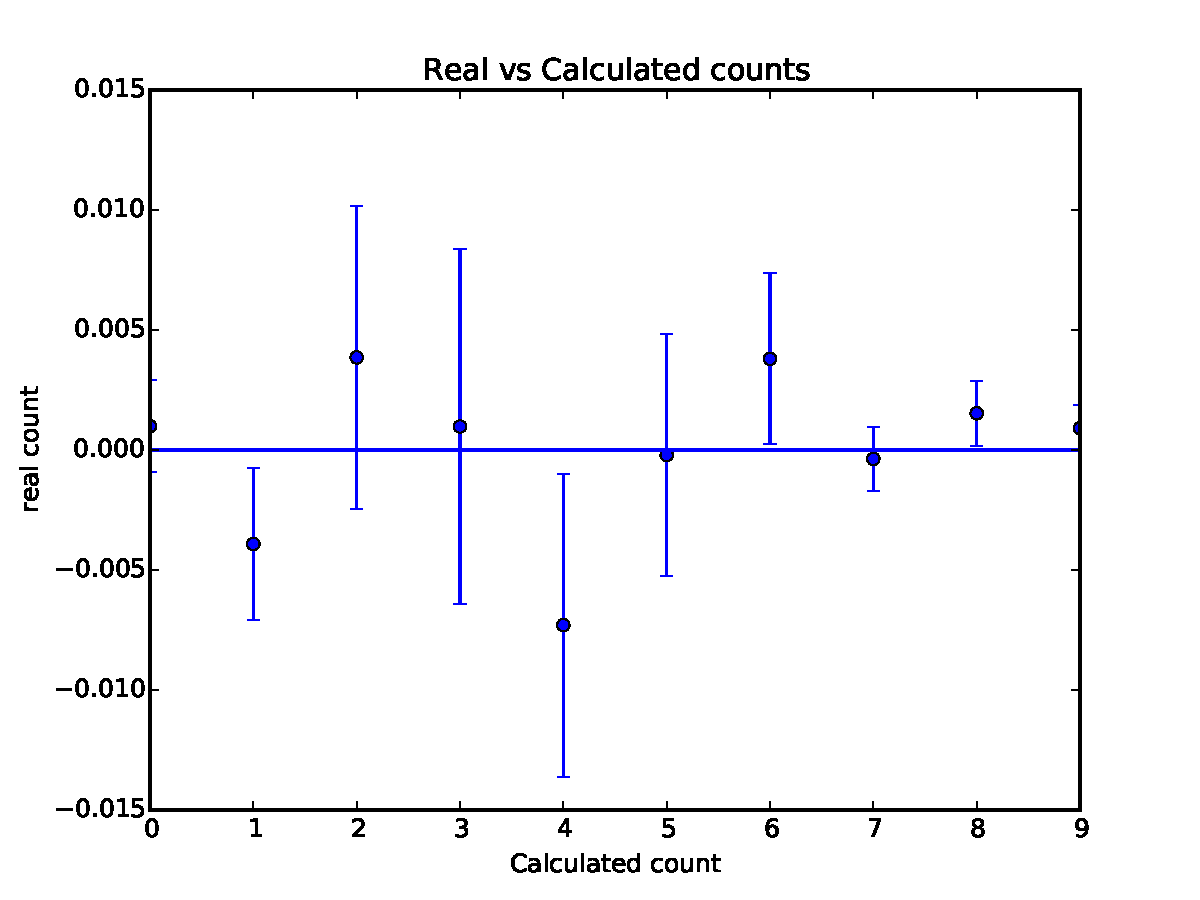
\includegraphics[height=10cm]{errorcomp.pdf}
\caption{Comparison of errors}
\label{errorcomp}
\end{center}
\end{figure}

 We found that all the bin counts were within 2 standard deviations, and all but 3 were within a single standard deviation, indicating both a good model fit and good estimation of errors.
    
\section{Summary}

The distribution was found to agree with a Poisson distribution in both numerical and perceptual measurements. A expected number of bins were more than 1 standard deviation from the Poisson distribution fitted to the mean of the data set as shown in Figure figure \ref{errorcomp}, and the shape of the curve was correct this model as shown in Figure \ref{curve}. 

To further evaluate this model, a modified experiment using a separate training and evaluation data set could be used to eliminate the chance of overfitting to the data. This is because the function that would best fit the binned data set would be a Lagrange polynomial of order 10. Despite the obvious non-physicality of a probability function for a simple system being described by a order 10 polynomial, this function would fit this data set perfectly and exhibit no error. using a separate training set would prevent this overfitting.

\clearpage
\printbibliography
\end{document}

